%%%%% Design %%%%%
\chapter{Contribution Statement}
\noindent \textbf{Zehao Ye}: In the group project, I make the overall project management as the group leader. Afterwards, I 
help my group members to config the environment for GitHub and LaTex usage. Besides, I complete the algorithm derivations 
related to forward kinematics, workspace simulations, angular conversion, inverse kinematics and trajectory replications, 
and these algorithms have been successfully developed and tested in both MATLAB and Python versions. Analysis has been made on these programmes. 
Meanwhile, I am also responsible for maintaining the GitHub repository and Documentation. \\
\qquad \\
\hspace*{\fill} Signature: \hrulefill
\vspace{-18mm}
\begin{center}
    \hspace{100mm}
    
\includegraphics[width=4cm]{Image/Signature/yezh.png} 
\end{center}
\qquad \\
\qquad \\
\noindent \textbf{Dawei Xu}: In this project, I was primarily responsible for conducting the structural strength analysis of the 
manipulator to ensure the reliability of the design. Additionally, I devoted substantial effort to the creation and optimization 
of CAD models, aiming to enhance structural efficiency and reduce potential weaknesses.  \\
\qquad \\
\hspace*{\fill} Signature: \hrulefill
\vspace{-17mm}
\begin{center}
    \hspace{100mm}
    
\includegraphics[width=4cm]{Image/Signature/xudw.png} 
\end{center}
\qquad \\
\qquad \\
\noindent \textbf{Jiachen Wu}: My main responsibilities were the structural design and material selection of the manipulator, 
sizing it and drawing up the CAD model, and I considered the sustainability of the product, as well as assisting Dawei with 
the strength verification and finite element analysis of the manipulator. In this paper I wrote the Design section and the 
Sustainability section. \\
\qquad \\
\hspace*{\fill} Signature: \hrulefill
\vspace{-15mm}
\begin{center}
    \hspace{100mm}
    
\includegraphics[width=4cm]{Image/Signature/wujc.png} 
\end{center}
\qquad \\
\noindent \textbf{Yuantong Li}: I have completed the actuation control part, including choosing the electronic components, 
designing the layout for control circuit and writing the Arduino control programme. The methodology and result for this part 
is illustrated in the corresponding sections in the report. \\
\qquad \\
\hspace*{\fill} Signature: \hrulefill
\vspace{-18mm}
\begin{center}
    \hspace{100mm}
    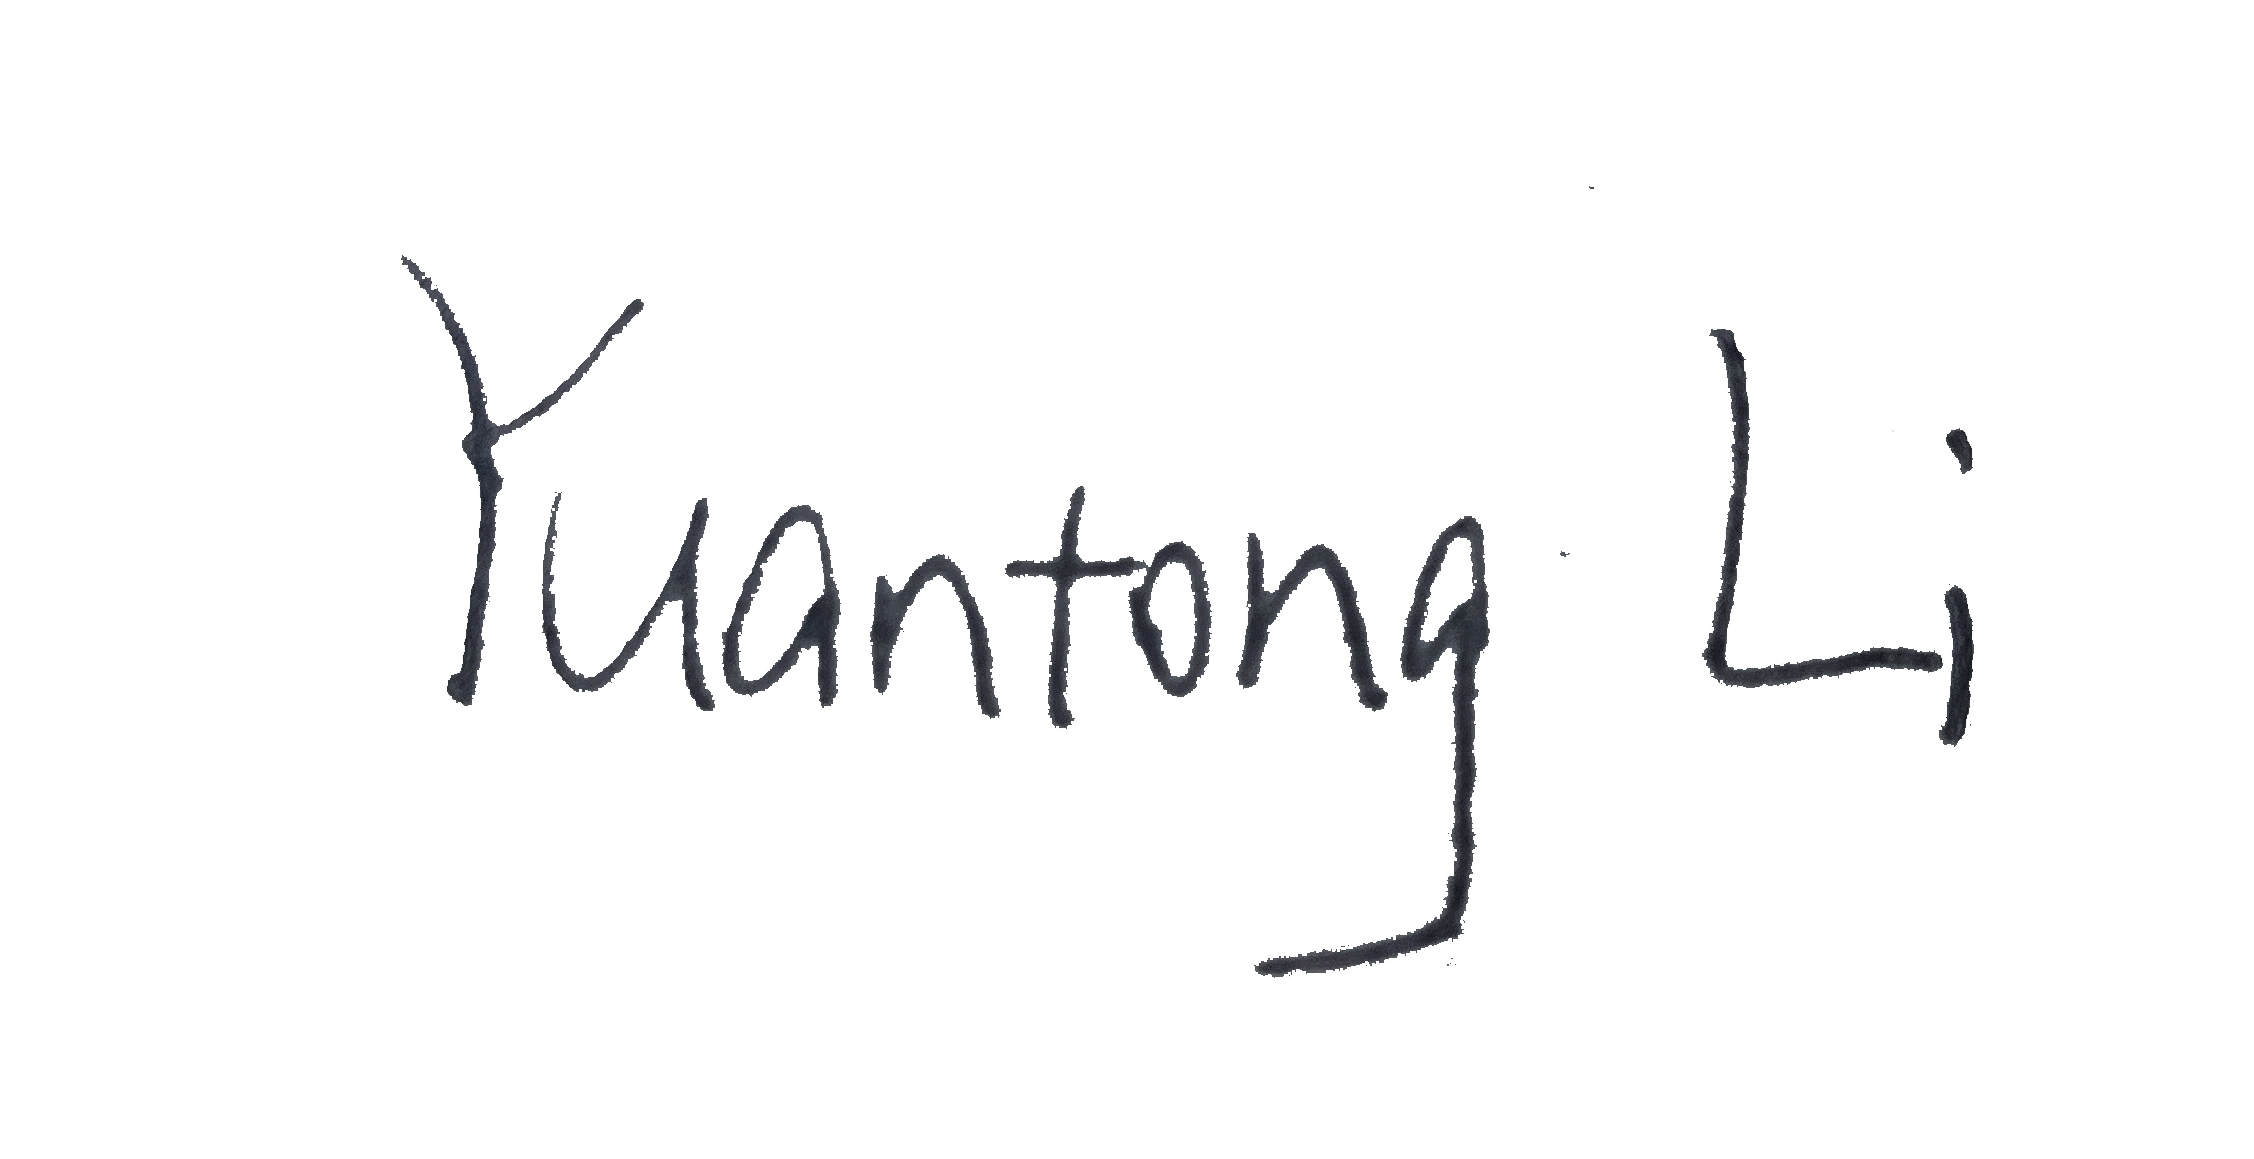
\includegraphics[width=4cm]{Image/Signature/liyt.png} 
\end{center}
\qquad \\
\noindent \textbf{Yuehan Zhang}: In the group project, I completed the sensing and control part. This included selecting 
sensors, display screens, physical part verification, circuit simulation, and microcontroller embedded programming.
In addition, I assisted in part of the mechanical design, including a part of CAD modelling and simulation. \\
\qquad \\
\hspace*{\fill} Signature: \hrulefill
\vspace{-15mm}
\begin{center}
    \hspace{100mm}
    
\includegraphics[width=4cm]{Image/Signature/zhangyh.png} 
\end{center}
\qquad \\
\noindent \textbf{Yuhao Zhu}: In the group project, I have contributed to the analysis of the physical model which contributes 
to the initial understanding of errors calculation \& analysis and forward kinematics. I also cooperated with Zehao to develop 
the MATLAB code for workspace simulation and forward kinematics. In the final stage of the project, I analyzed the results of 
both error calculations and workspace simulation, besides I also derived the function of changes of driving cables against the 
bending angles and demonstrated the process in project report. \\
\qquad \\
\hspace*{\fill} Signature: \hrulefill
\vspace{-20mm}
\begin{center}
    \hspace{100mm}
    
\includegraphics[width=4cm]{Image/Signature/zhuyh.png} 
\end{center}
\qquad \\



% change to new page
\newpage